\documentclass[border=0,tikz]{standalone}
\usepackage{amsmath}
\usetikzlibrary{arrows}
\usetikzlibrary{intersections}
\usetikzlibrary{calc}

\begin{document}
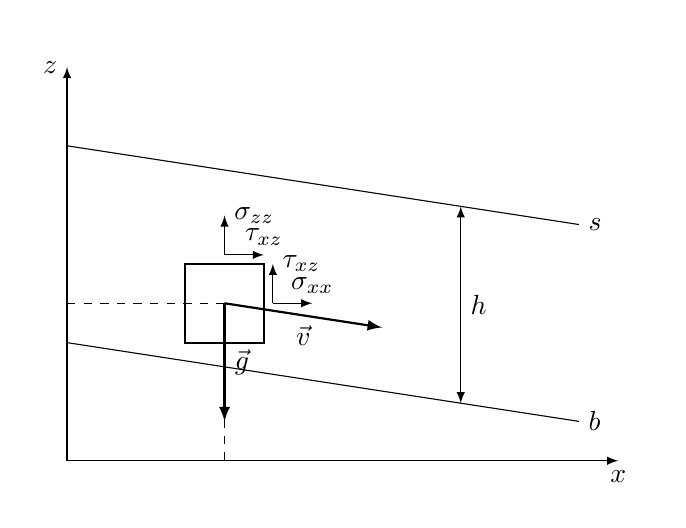
\begin{tikzpicture}[>=latex]

% background and axes
\fill[white] (-0.5,-0.5) rectangle +(8,6);
%\draw [help lines, lightgray] (0,0) grid (7,5);
\draw[->] (0,0) -- (7,0) node [below] {$x$};
\draw[->] (0,0) -- (0,5) node [left] {$z$};

% surface and bed profiles
\draw[name path=s] (0,4) -- (6.5,3) node [right] {$s$};
\draw[name path=b] (0,1.5) -- (6.5,0.5) node [right] {$b$};

% central point coordinates
\coordinate (p) at (2,2);
\draw[dashed] (p |- 0,0) -- (p);
\draw[dashed] (p -| 0,0) -- (p);

% velocity and gravity vectors
\draw[->, thick] (p) -- +(2,-1/3.25) node [midway, below] {$\vec{v}$};
\draw[->, thick] (p) -- +(0,-1.5) node [midway, right] {$\vec{g}$};

% stress tensor cube
\node (box) at (p) [rectangle,draw,thick,minimum size=10mm] {};
\draw[->] (box.north) ++(0,0.1) -- ++(0,0.5) node [right] {$\sigma_{zz}$};
\draw[->] (box.north) ++(0,0.1) -- ++(0.5,0) node [above] {$\tau_{xz}$};
\draw[->] (box.east) ++(0.1,0) -- ++(0,0.5) node [right] {$\tau_{xz}$};
\draw[->] (box.east) ++(0.1,0) -- ++(0.5,0) node [above] {$\sigma_{xx}$};

% ice thickness
\path [name path=hx] (5,0) -- +(0,5);
\path [name intersections={of=s and hx, by=hs}] ;
\path [name intersections={of=b and hx, by=hb}] ;
\draw[<->] (hb) -- (hs) node [midway, right] {$h$};

\end{tikzpicture}
\end{document}
